% This file was converted to LaTeX by Writer2LaTeX ver. 1.0.2
% see http://writer2latex.sourceforge.net for more info
\documentclass[twoside,letterpaper]{article}
\usepackage[latin1]{inputenc}
\usepackage[T1]{fontenc}
\usepackage[english]{babel}
\usepackage{amsmath}
\usepackage{amssymb,amsfonts,textcomp}
\usepackage{color}
\usepackage{array}
\usepackage{supertabular}
\usepackage{hhline}
\usepackage{hyperref}
\hypersetup{pdftex, colorlinks=true, linkcolor=blue, citecolor=blue, filecolor=blue, urlcolor=blue, pdftitle=SYSTEM AND SOFTWARE ARCHITECTURAL AND DETAILED DESIGN DESCRIPTI, pdfauthor=Clinton Jeffery, pdfsubject=, pdfkeywords=}
\usepackage[pdftex]{graphicx}

% multiline comment
\usepackage{verbatim}

% Outline numbering
\setcounter{secnumdepth}{5}
\renewcommand\thesection{\arabic{section}}
\renewcommand\thesubsection{\arabic{section}.\arabic{subsection}}
\renewcommand\thesubsubsection{\arabic{section}.\arabic{subsection}.\arabic{subsubsection}}
\renewcommand\theparagraph{\arabic{section}.\arabic{subsection}.\arabic{subsubsection}.\arabic{paragraph}}
\renewcommand\thesubparagraph{\arabic{section}.\arabic{subsection}.\arabic{subsubsection}.\arabic{paragraph}.\arabic{subparagraph}}
\makeatletter
\newcommand\arraybslash{\let\\\@arraycr}
\makeatother
% List styles
\newcommand\liststyleWWviiiNumii{%
\renewcommand\theenumi{\arabic{enumi}}
\renewcommand\theenumii{\arabic{enumii}}
\renewcommand\theenumiii{\arabic{enumiii}}
\renewcommand\theenumiv{\arabic{enumiv}}
\renewcommand\labelenumi{\theenumi)}
\renewcommand\labelenumii{\theenumii.}
\renewcommand\labelenumiii{\theenumiii.}
\renewcommand\labelenumiv{\theenumiv.}
}
% Page layout (geometry)
\setlength\voffset{-1in}
\setlength\hoffset{-1in}
\setlength\topmargin{0.5in}
\setlength\oddsidemargin{1in}
\setlength\evensidemargin{1in}
\setlength\textheight{8.278in}
\setlength\textwidth{6.5in}
\setlength\footskip{0.561in}
\setlength\headheight{0.5in}
\setlength\headsep{0.461in}
% Footnote rule
\setlength{\skip\footins}{0.0469in}
\renewcommand\footnoterule{\vspace*{-0.0071in}\setlength\leftskip{0pt}\setlength\rightskip{0pt plus 1fil}\noindent\textcolor{black}{\rule{0.25\columnwidth}{0.0071in}}\vspace*{0.0398in}}
% Pages styles
\makeatletter
\newcommand\ps@Standard{
  \renewcommand\@oddhead{}
  \renewcommand\@evenhead{\@oddhead}
  \renewcommand\@oddfoot{\foreignlanguage{english}{\textcolor{black}{\hfill SSDD Page }}{\textcolor{black}{\thepage{}}}}
  \renewcommand\@evenfoot{\@oddfoot}
  \renewcommand\thepage{\arabic{page}}
}
\newcommand\ps@Convertix{
  \renewcommand\@oddhead{}
  \renewcommand\@evenhead{\@oddhead}
  \renewcommand\@oddfoot{}
  \renewcommand\@evenfoot{\@oddfoot}
  \renewcommand\thepage{\arabic{page}}
}
\newcommand\ps@Convertviii{
  \renewcommand\@oddhead{}
  \renewcommand\@evenhead{\@oddhead}
  \renewcommand\@oddfoot{}
  \renewcommand\@evenfoot{\@oddfoot}
  \renewcommand\thepage{\arabic{page}}
}
\newcommand\ps@Convertvii{
  \renewcommand\@oddhead{}
  \renewcommand\@evenhead{\@oddhead}
  \renewcommand\@oddfoot{}
  \renewcommand\@evenfoot{\@oddfoot}
  \renewcommand\thepage{\arabic{page}}
}
\newcommand\ps@Convertvi{
  \renewcommand\@oddhead{}
  \renewcommand\@evenhead{\@oddhead}
  \renewcommand\@oddfoot{}
  \renewcommand\@evenfoot{\@oddfoot}
  \renewcommand\thepage{\arabic{page}}
}
\newcommand\ps@Convertiv{
  \renewcommand\@oddhead{}
  \renewcommand\@evenhead{\@oddhead}
  \renewcommand\@oddfoot{}
  \renewcommand\@evenfoot{\@oddfoot}
  \renewcommand\thepage{\arabic{page}}
}
\newcommand\ps@FirstPage{
  \renewcommand\@oddhead{}
  \renewcommand\@evenhead{\@oddhead}
  \renewcommand\@oddfoot{\foreignlanguage{english}{\textcolor{black}{\hfill SSDD Page }}
{\textcolor{black}{\thepage{}}}}
  \renewcommand\@evenfoot{\@oddfoot}
  \renewcommand\thepage{\arabic{page}}
}
\makeatother
\pagestyle{Standard}
\setlength\tabcolsep{1mm}
\renewcommand\arraystretch{1.3}
\title{SYSTEM AND SOFTWARE ARCHITECTURAL AND DETAILED DESIGN DESCRIPTION}
\author{Clinton Jeffery}
\date{2010-11-18T11:30:10.24}
\begin{document}

%% %% %% %% %% %% %% %% %% %% %% %% %% %% %% %% %% %% %% %% %% %% %% %% %% %% 
\begin{comment}
\clearpage\setcounter{page}{1}\pagestyle{Standard}
\thispagestyle{FirstPage}
{\centering\selectlanguage{english}\bfseries\color{black}
SYSTEM AND SOFTWARE\newline
DESIGN DESCRIPTION (SSDD) TEMPLATE
\par}

{\centering\selectlanguage{english}\bfseries\color{black}
(Incorporating Architectural Views and Detailed Design Criteria)
\par}

{\centering\selectlanguage{english}\bfseries\color{black}
Version A.2, November 2010
\par}

{\centering\selectlanguage{english}\bfseries\color{black}
FOREWORD
\par}

{\selectlanguage{english}\color{black}
This template was created to provide system and software development
projects with a model System and Software Design Description (SSDD)
that incorporates both architectural views and detailed design
criteria. \ The template is based on work compiled by Dr.~Paul Oman
from a large collection of software engineering design document
standards discussed in Section 1.5. \ It has been edited and updated by
Dr.~Clint Jeffery for use in UI CS 383.}

{\selectlanguage{english}\color{black}
The SSDD template begins on the next page. \ Just throw away this page
and enter your project specifications into the following template.
\ Don{\textquoteright}t forget to change the headers and footers as
necessary. \ The following conventions are used to guide you in
developing your SSDD:}

\bigskip

\end{comment}
%% %% %% %% %% %% %% %% %% %% %% %% %% %% %% %% %% %% %% %% %% %% %% %% %% %% 
\clearpage

{\centering\selectlanguage{english}\bfseries\color{black}
SYSTEM AND SOFTWARE DESIGN DESCRIPTION (SSDD): Incorporating
Architectural Views and Detailed Design Criteria
\par}

{\centering\selectlanguage{english}\bfseries\color{black}
FOR
\par}


\bigskip

{\centering\selectlanguage{english}\bfseries\color{black}
Project: UML
\par}


\bigskip


\bigskip


\bigskip

{\centering \par}

\begin{figure}
\centering

\includegraphics[scale=3]{viking.png}
\end{figure}

\bigskip


\bigskip


\bigskip


\bigskip

{\centering\selectlanguage{english}\bfseries\color{black}
Version 1.1
\par}

{\centering\selectlanguage{english}\bfseries\color{black}
[12/16/2011]
\par}


\bigskip


\bigskip

{\centering\selectlanguage{english}\bfseries\color{black}
Prepared for:
\par}

{\centering\selectlanguage{english}\bfseries\color{black}
Professor Bruce Bolden, Dr. Clinton Jeffery
\par}


\bigskip


\bigskip

{\centering\selectlanguage{english}\bfseries\color{black}
Prepared by:
\par}

{\centering\selectlanguage{english}\bfseries\color{black}
Coleman Beasley, Alex Dean, Austin Enfield, Jason Fletcher, Theora Rice, Cable Johnson, Adrian Norris, David Summers
\par}

\bigskip

{\centering\selectlanguage{english}\bfseries\color{black}
Emeritus Contributors:
\par}

{\centering\selectlanguage{english}\bfseries\color{black}
Noel Klein, Max McKinnon
\par}

\bigskip
\bigskip

{\centering\selectlanguage{english}\bfseries\color{black}
University of Idaho
\par}

{\centering\selectlanguage{english}\bfseries\color{black}
Moscow, ID \ 83844-1010
\par}

\clearpage{\centering\selectlanguage{english}\bfseries\color{black}
CS383 SSDD
\par}

{\centering\selectlanguage{english}\bfseries\color{black}
RECORD OF CHANGES (Change History) (N/A)
\par}

\begin{flushleft}
\tablehead{}
\begin{supertabular}{|m{0.5462598in}|m{0.6712598in}|m{1.4212599in}|m{0.23375985in}|m{1.7962599in}|m{0.7337598in}|m{0.6295598in}|}
\hline
~

\centering {\selectlanguage{english}\bfseries\color{black} Change}\par

\centering {\selectlanguage{english}\bfseries\color{black} Number}\par

~
 &
~

\centering \selectlanguage{english}\bfseries\color{black} Date completed
&
~

\centering {\selectlanguage{english}\bfseries\color{black} Location of
change }\par

\centering \selectlanguage{english}\bfseries\color{black} (e.g., page or
figure \#) &
~

\centering {\selectlanguage{english}\bfseries\color{black} A}\par

\centering \selectlanguage{english}\bfseries\color{black} M\newline
D  &
~

\centering {\selectlanguage{english}\bfseries\color{black} Brief
description }\par

\centering \selectlanguage{english}\bfseries\color{black} of change &
~

\centering \selectlanguage{english}\bfseries\color{black} Approved by
(initials) &
~

\centering {\selectlanguage{english}\bfseries\color{black} Date }\par

\centering\arraybslash \selectlanguage{english}\bfseries\color{black}
approved\\\hline
01
 &
2012.02.02
 &
line 1107
 &
A
 &
Added class diagram based on current code.
 &
DS
 &
~
\\\hline
~
 &
~
 &
~
 &
~
 &
~
 &
~
 &
~
\\\hline
~
 &
~
 &
~
 &
~
 &
~
 &
~
 &
~
\\\hline
~
 &
~
 &
~
 &
~
 &
~
 &
~
 &
~
\\\hline
~
 &
~
 &
~
 &
~
 &
~
 &
~
 &
~
\\\hline
~
 &
~
 &
~
 &
~
 &
~
 &
~
 &
~
\\\hline
~
 &
~
 &
~
 &
~
 &
~
 &
~
 &
~
\\\hline
~
 &
~
 &
~
 &
~
 &
~
 &
~
 &
~
\\\hline
~
 &
~
 &
~
 &
~
 &
~
 &
~
 &
~
\\\hline
~
 &
~
 &
~
 &
~
 &
~
 &
~
 &
~
\\\hline
~
 &
~
 &
~
 &
~
 &
~
 &
~
 &
~
\\\hline
~
 &
~
 &
~
 &
~
 &
~
 &
~
 &
~
\\\hline
~
 &
~
 &
~
 &
~
 &
~
 &
~
 &
~
\\\hline
~
 &
~
 &
~
 &
~
 &
~
 &
~
 &
~
\\\hline
~
 &
~
 &
~
 &
~
 &
~
 &
~
 &
~
\\\hline
~
 &
~
 &
~
 &
~
 &
~
 &
~
 &
~
\\\hline
~
 &
~
 &
~
 &
~
 &
~
 &
~
 &
~
\\\hline
~
 &
~
 &
~
 &
~
 &
~
 &
~
 &
~
\\\hline
~
 &
~
 &
~
 &
~
 &
~
 &
~
 &
~
\\\hline
~
 &
~
 &
~
 &
~
 &
~
 &
~
 &
~
\\\hline
~
 &
~
 &
~
 &
~
 &
~
 &
~
 &
~
\\\hline
~
 &
~
 &
~
 &
~
 &
~
 &
~
 &
~
\\\hline
\end{supertabular}
\end{flushleft}
{\selectlanguage{english}\color{black}
A - ADDED \ M - MODIFIED \ D -- DELETED}

\clearpage{\centering\selectlanguage{english}\bfseries\color{black}
PUML
\par}

{\centering\selectlanguage{english}\bfseries\color{black}
TABLE OF CONTENTS
\par}

{\selectlanguage{english}\bfseries\color{black}
Section\ \ Page}

\setcounter{tocdepth}{9}
\renewcommand\contentsname{}
\tableofcontents

\bigskip

\bigskip
\clearpage\setcounter{page}{1}\pagestyle{Convertiv}
\section[INTRODUCTION (Alex)]{\selectlanguage{english}\bfseries\color{black}
INTRODUCTION (Alex)}

\subsection{IDENTIFICATION}

{\selectlanguage{english}\color{black}
		This document describes the first version of pUML.  pUML is a UML diagram drawing tool that will operate under any system able to compile it with QT Creator 4.7.}

\subsection[DOCUMENT PURPOSE, SCOPE, AND INTENDED
AUDIENCE]{\selectlanguage{english}\bfseries\color{black} DOCUMENT
PURPOSE, SCOPE, AND INTENDED AUDIENCE}


\subsubsection{Document Purpose}
{\selectlanguage{english}\color{black}
		This Software Design Document provides the design details of Project Unified Modeling Language (pUML).
}

\subsubsection{Document Scope and/or Context}
{\selectlanguage{english}\color{black}
		This document contains a complete description of the design of pUML.  The project is written with C++ and the Qt framework. The project leader designated is Coleman Beasley.  He will have full access to make changes as he deems necessary.
}

\subsubsection{Intended Audience for Document}
{\selectlanguage{english}\color{black}
	The intended audience is Bruce Bolden, the pUML developers, and the people who maintain pUML.
}

\subsection[SYSTEM AND SOFTWARE PURPOSE, SCOPE, AND INTENDED
USERS]{\selectlanguage{english}\bfseries\color{black} SYSTEM AND
SOFTWARE PURPOSE, SCOPE, AND INTENDED USERS}

\subsubsection{System and Software Purpose}
{\selectlanguage{english}\color{black}
		This software provides the user with a quick and efficient means to construct high quality UML diagrams.}

\subsubsection[System and Software Scope/or Context]{System and Software
Scope/or Context}
{\selectlanguage{english}\color{black}
		The scope of this application is provide the user with a means to construct high quality UML diagrams.  This includes implementing the following features at a minimum:
		\begin{list}{-}{spacing}
		\item All shapes needed for standard UML diagrams (including an actor shape)
		\item Line objects for creating connections
		\item Text areas to write comments for the diagrams
		\item Ability to save and load projects
		\item Exportability to PDF format
		\end{list}
}

\subsubsection{Intended Users for the System and Software}
{\selectlanguage{english}\color{black}
		The intended users for this application are students and professionals seeking an advanced tool to construct a UML diagram.
}

\subsection[DEFINITIONS, ACRONYMS, AND
ABBREVIATIONS]{\selectlanguage{english}\bfseries\color{black}
DEFINITIONS, ACRONYMS, AND ABBREVIATIONS}

\bigskip

\begin{flushleft}
\tablehead{\hline
\centering \selectlanguage{english}\bfseries\color{black} Term or
Acronym &
\centering\arraybslash \selectlanguage{english}\bfseries\color{black}
Definition\\\hline}
\begin{supertabular}{|m{1.3587599in}|m{5.00806in}|}
\selectlanguage{english}\color{black} Acquirer &
\selectlanguage{english}\color{black} The person, team, or organization
that pursues a system or software product or service from a supplier.
The acquirer may be a buyer, customer, owner, purchaser, or user.
\ ISO/IEC 42010:2007 (�3.1).\\\hline
\selectlanguage{english}\color{black} AD &
\selectlanguage{english}\color{black} Architectural Description:
{\textquotedblleft}A collection of products to document an
architecture{\textquotedblright} ISO/IEC 42010:2007 (�3.4).\\\hline
\selectlanguage{english}\color{black} Alpha test &
\selectlanguage{english}\color{black} Limited release(s) to selected,
outside testers\\\hline
\selectlanguage{english}\color{black} Architect &
\selectlanguage{english}\color{black}
\foreignlanguage{english}{{\textquotedblleft}}\foreignlanguage{english}{The
person, team, or organization responsible for systems
architecture{\textquotedblright} ISO/IEC 42010:2007 (�3.2).}\\\hline
\selectlanguage{english}\color{black} Architectural Description &
\selectlanguage{english}\color{black} (AD) {\textquotedblleft}A
collection of products to document an architecture{\textquotedblright}
ISO/IEC 42010:2007 (�3.4).\\\hline
\selectlanguage{english}\color{black} Architectural View &
\selectlanguage{english}\color{black}
\foreignlanguage{english}{{\textquotedblleft}}\foreignlanguage{english}{A
representation of a whole system from the perspective of a related set
of concerns{\textquotedblright} ISO/IEC 42010:2007 (�3.9).}\\\hline
\selectlanguage{english}\color{black} Architecture &
\selectlanguage{english}\color{black}
\foreignlanguage{english}{{\textquotedblleft}}\foreignlanguage{english}{The
fundamental organization of a system embodied in its components, their
relationships to each other, and to the environment, and the principles
guiding its design and evolution{\textquotedblright} ISO/IEC 42010:2007
(�3.5).}\\\hline
\selectlanguage{english}\color{black} Beta test &
\selectlanguage{english}\color{black} Limited release(s) to cooperating
customers wanting early access to developing systems\\\hline
\selectlanguage{english}\color{black} Design Entity &
\selectlanguage{english}\color{black}
\foreignlanguage{english}{{\textquotedblleft}}\foreignlanguage{english}{An
element (component) of a design that is structurally and functionally
distinct from other elements and that is separately named and
referenced{\textquotedblright} IEEE STD 1016-1998 (�3.1).}\\\hline
\selectlanguage{english}\color{black} Design View &
\selectlanguage{english}\color{black}
\foreignlanguage{english}{{\textquotedblleft}}\foreignlanguage{english}{A
subset of design entity attribute information that is specifically
suited to the needs of a software project activity{\textquotedblright}
IEEE STD 1016-1998 (�3.2).}\\\hline
\selectlanguage{english}\color{black} Final test &
\selectlanguage{english}\color{black} aka, Acceptance test, release of
full functionality to customer for approval\\\hline
\selectlanguage{english}\color{black} DFD &
\selectlanguage{english}\color{black} Data Flow Diagram\\\hline
\selectlanguage{english}\color{black} SDD &
\selectlanguage{english}\color{black} Software Design Document, aka SDS,
Software Design Specification\\\hline
\selectlanguage{english}\color{black} Software Design Description &
\selectlanguage{english}\color{black}
\foreignlanguage{english}{{\textquotedblleft}}\foreignlanguage{english}{A
representation of a software system created to facilitate analysis,
planning, implementation, and decision making, A blueprint or model of
a software system. The SDD is used as the primary medium for
communicating software }\foreignlanguage{english}{design
information{\textquotedblright} IEEE STD 1016-1998 (�3.4).}\\\hline
\selectlanguage{english}\color{black} SRS &
\selectlanguage{english}\color{black} Software Requirements
Specification\\\hline
\selectlanguage{english}\color{black} SSDD &
\selectlanguage{english}\color{black} System and Software Design
Document\\\hline
\selectlanguage{english}\color{black} SSRS &
\selectlanguage{english}\color{black} System and Software Requirements
Specification\\\hline
\selectlanguage{english}\color{black} System &
\selectlanguage{english}\color{black}
\foreignlanguage{english}{{\textquotedblleft}}\foreignlanguage{english}{A
collection of components organized to accomplish a specific function or
set of functions{\textquotedblright} ISO/IEC 42010:2007
(�3.7).}\\\hline
\selectlanguage{english}\color{black} System and Software Architecture
and Design Description &
\selectlanguage{english}\color{black} An architectural and detailed
design description that includes a software system within the context
of its enclosing system and describes the enclosing system, the
enclosed software, and their relationship and interfaces.\\\hline
\selectlanguage{english}\color{black} System Stakeholder &
\selectlanguage{english}\color{black}
\foreignlanguage{english}{{\textquotedblleft}}\foreignlanguage{english}{An
individual, team, or organization (or classes thereof) with interests
in, or concerns, relative to, a system{\textquotedblright} ISO/IEC
42010:2007 (�3.8).}\\\hline
~
 &
~
\\\hline
~
 &
~
\\\hline
\end{supertabular}
\end{flushleft}
\subsection[DOCUMENT
REFERENCES]{\selectlanguage{english}\bfseries\color{black} DOCUMENT
REFERENCES}
\liststyleWWviiiNumii
\begin{enumerate}
\item {\selectlanguage{english}\color{black}
\foreignlanguage{english}{CSDS,
}\foreignlanguage{english}{\textit{System and Software Requirements
Specification Template}}\foreignlanguage{english}{, Version 1.0, July
31, 2008, Center for Secure and Dependable Systems, University of
Idaho, Moscow, ID, 83844.}}
\item {\selectlanguage{english}\color{black}
\foreignlanguage{english}{ISO/IEC/IEEE,
}\foreignlanguage{english}{\textit{IEEE Std 1471-2000 Systems and
software engineering -- Recommended practice for architectural
description of software intensive systems,}}\foreignlanguage{english}{
First edition 2007-07-15, \ International Organization for
Standardization and International Electrotechnical Commission,
(ISO/IEC), Case postale 56, CH-1211 Gen�ve 20, Switzerland, and The
Institute of Electrical and Electronics Engineers, Inc., (IEEE), 445
Hoes Lane, Piscataway, NJ 08854, USA.}}
\item {\selectlanguage{english}\color{black}
\foreignlanguage{english}{IEEE, }\foreignlanguage{english}{\textit{IEEE
Std 1016-1998 Recommended Practice for Software Design
Descriptions}}\foreignlanguage{english}{, 1998-09-23, The Institute of
Electrical and Electronics Engineers, Inc., (IEEE) 445 Hoes Lane,
Piscataway, NJ 08854, USA.}}
\item {\selectlanguage{english}\color{black}
\foreignlanguage{english}{3) ISO/IEC/IEEE,
}\foreignlanguage{english}{\textit{IEEE Std. 15288-2008 Systems and
Software Engineering -- System life cycle
processes,}}\foreignlanguage{english}{ Second edition 2008-02-01,
\ International Organization for Standardization and International
Electrotechnical Commission, (ISO/IEC), Case postale 56, CH-1211 Gen�ve
20, Switzerland, and The Institute of Electrical and Electronics
Engineers, Inc., (IEEE), 445 Hoes Lane, Piscataway, NJ 08854, USA.}}
\item {\selectlanguage{english}\color{black}
\foreignlanguage{english}{ISO/IEC/IEEE, IEEE Std. 12207-2008,
}\foreignlanguage{english}{\textit{Systems and software engineering --
Software life cycle processes, }}\foreignlanguage{english}{Second
edition 2008-02-01, \ International Organization for Standardization
and International Electrotechnical Commission, (ISO/IEC), Case postale
56, CH-1211 }\foreignlanguage{english}{Gen�ve 20, Switzerland, and The
Institute of Electrical and Electronics Engineers, Inc., (IEEE), 445
Hoes Lane, Piscataway, NJ 08854, USA.}}
\end{enumerate}
	6) Qt Development Frameworks Documentation. [Online] Available: http://doc.qt.nokia.com/
6) Qt Development Frameworks Documentation. [Online] Available: http://doc.qt.nokia.com/

\subsection{DOCUMENT OVERVIEW}
{\selectlanguage{english}\color{black}
Section 2 of this document describes the system and software constraints
imposed by the operational environment, system requirements and user
characteristics, and then identifies the system stakeholders and lists
describes their concerns and mitigations to those concerns.}

{\selectlanguage{english}\color{black}
Section 3 of this document describes the system and software
architecture from several viewpoints, including, but not limited to,
the developer{\textquoteright}s view and the user{\textquoteright}s
view.}

{\selectlanguage{english}\color{black}
Section 4 provides detailed design descriptions for every component
defined in the architectural view(s). \ Sections 5 provides
traceability information connecting the original specifications
(referenced above) to the architectural components and design entities
identified in this document.}

{\selectlanguage{english}\color{black}
Section 6 and beyond are appendices including original information and
communications used to create this document.}

\subsection[DOCUMENT
RESTRICTIONS]{\selectlanguage{english}\bfseries\color{black} DOCUMENT
RESTRICTIONS}

{\selectlanguage{english}\color{black}
	This document is for LIMITED RELEASE ONLY to UI CS personnel working on the project, Bruce Bolden, and his associates.}

% The following section was edited by noel
\section{CONSTRAINTS (Noel)}
{\selectlanguage{english}\itshape\color{black}
This section identifies and describes in detail the architectural
and usability constraints that are imposed by the physical environment
and system requirements and the user characteristics.}

\subsection{Environmental constraints.}
{\selectlanguage{english}\color{black}
The tool can be used in every environment that satisfies the system requirements defined in the next subsection. Since it is a software design tool, it will most likely be in a software design environment.}

\subsection{System requirement constraints.}
{\selectlanguage{english}\color{black}
The tool requires normal x86 hardware and runs on Windows, Mac OSX, and Linux.}

\subsection{User characteristic constraints.}
{\selectlanguage{english}\color{black}
It is a tool that supports the creation of UML diagrams and therefore requires the knowledge of how UML diagrams work. }

% Noel end
\clearpage\setcounter{page}{1}\pagestyle{Convertvi}
\section[SYSTEM AND SOFTWARE
ARCHITECTURE (Theora)]{\selectlanguage{english}\bfseries\color{black} SYSTEM AND
SOFTWARE ARCHITECTURE (Theora)}


\subsection{DEVELOPER{\textquoteright}S ARCHITECTURAL VIEW}
\subparagraph*{}
{\selectlanguage{english}\color{black}
From the developer{\textquoteright}s point of view, the architecture is modular, based around separate tool bars and 
windows gathered around a single menu. 
It has been written in C++. The Drawing Area module is where the events of the program are centred 
and displayed. It uses different methods for mouse-movement and dragging events. It also contains 
a paint method to illustrate the final output shape. The objects it displays come from the objects class, 
which holds the various subclasses that contain each shape. Each of these subclasses contains only 
their own creation method. }


\begin{comment}
\subsection[DEVELOPER{\textquoteright}S ARCHITECTURAL
VIEW]{\selectlanguage{english}\bfseries\color{black}
DEVELOPER{\textquoteright}S ARCHITECTURAL VIEW}
\subparagraph*{{\selectlanguage{english}\color{black}
From the developer{\textquoteright}s point of view, the architecture is modular, based around separate tool bars and 
windows gathered around a single menu. 
It has been written in C++. The Drawing Area module is where the events of the program are centred 
and displayed. It uses different methods for mouse-movement and dragging events. It also contains 
a paint method to illustrate the final output shape. The objects it displays come from the objects class, 
which holds the various subclasses that contain each shape. Each of these subclasses contains only 
their own creation method. }
}
\end{comment}


\subparagraph*{}%{\selectlanguage{english}\color{black}
The Toolbar is the next most important module, as it controls the drawing of objects and their 
properties afterwards. It triggers inserting an object with the insertShape() and insertLine() methods, 
as well as contains the method that calls the OptionsDialog.%}}

\subparagraph*{}%{\selectlanguage{english}\color{black}
The Options Dialog  updates each shape object with the new user-chosen colours, text, and line weight. 
It is a user interface where they will be presented with a selection of options to choose from to modify 
their diagram.%}}

\subparagraph*{}%{\selectlanguage{english}\color{black}
Objects will be represented within one common class, that will contain links to each shape's individual 
subclass. These subclasses will contain the shape's properties such as position, colour, size, etc., 
as well as their own creation method.%}}

\subparagraph*{}%{\selectlanguage{english}\color{black}
The File Method contains any information about the file itself, and will default save the file to a 
database as an XML file. It also has open(), savePDF(), and BMP() for opening files and saving them 
to different formats. This will also contain the list of recent user actions for the undo and redo 
functionality. These actions will be kept in a linked list for reference.%}}

\subsection{USER{\textquoteright}S ARCHITECTURAL VIEW}
%{\selectlanguage{english}\bfseries\color{black}
%USER{\textquoteright}S ARCHITECTURAL VIEW}

\subparagraph*{}%{\selectlanguage{english}\color{black}
From the user{\textquoteright}s viewpoint, there are three separate modules: 
The Main Window, the Drawing Area, and the Toolbar. The Main Window will act
as background, which the other components will use to orient themselves.
This window will contain the file management buttons, such as save, open, 
undo, redo, and help.%}}

\subparagraph*{}%{\selectlanguage{english}\color{black}
The Drawing Area will be where users get to manipulate the individual objects and the 
overall diagram they create. The background will be a plain white drawing space, across which
 the users will be able to drag their objects. By left clicking each object, users will 
 be able to access the Options Dialogue box, where they will be able to change the line width, 
 fill colour (for non-lines,) font (for text boxes,) and line colour.  Thus, the Drawing Area 
 controls where one can put the shapes, the Options dialogue changes the shape's properties 
 and the shapes keep track of their own values.%}}

\subparagraph*{}%{\selectlanguage{english}\color{black}
The Toolbar allows the user to create shapes on the Drawing Area, and access the Options Dialogue 
box to change the default value of a shape before it is created. It will also be used to toggle 
the Grid on and off the Drawing Area.%}}

\subsection{User{\textquoteright}s View Identification}
%{\selectlanguage{english}\bfseries\color{black}
%User{\textquoteright}s View Identification}

\subparagraph*{}%{\selectlanguage{english}\color{black}
From the User's point of view, things are mostly GUI based for easy utilization. 
Within the top level of the architecture, the Main Window, there are file operation processes.
 The save button will summon a drop down menu that contains
buttons to (default) save the file as an XML document, export to PDF, export to 
BMP, and exit without saving. The open button will automatically bring up a directory 
dialogue so that the user can choose files. Undo will reverse the previous user 
action, and redo will reinstate it. The help button will contain a drop down menu
with buttons that summon the \textquotedblleft About\textquotedblright dialogue window
and the User Manual Dialogue. The About dialogue will display general information about the 
program and who created it. The User Manual Dialogue will contain the usual Help window, in 
which users can manipulate different tabs to get the information they need in order to use
the program.%}}

\subparagraph*{}%{\selectlanguage{english}\color{black}
The Drawing Area will contain the processes that allow for manipulation of the shapes and
diagram. By left clicking on a shape and holding down on the mouse button, the user can 
drag shapes across the background and change their coordinates. By dragging down on the 
bottom right hand corner  of these objects, users will be able to resize them.
 Multiple shapes can be selected by clicking on each in turn while holding the ctrl key.
 All above processes can be performed upon these group selected shapes as well.%}}

\subparagraph*{}{\selectlanguage{english}\color{black}
The Toolbar contains the processes that will be used to signal the creation of a shape, line, and text box. 
It also contains the ability to open the Options Dialogue, and the button to toggle the grid on and off.}%}

\subsubsection{User{\textquoteright}s View Representation and Description }
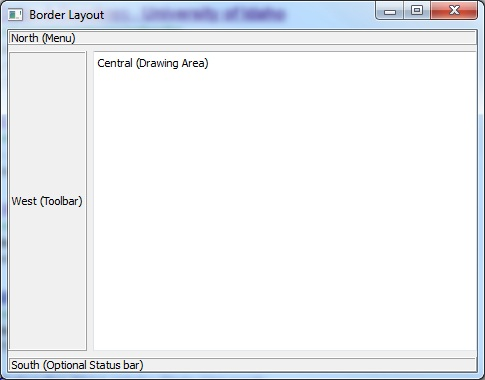
\includegraphics[scale=0.5]{Layout.png}
\\
{\selectlanguage{english}\color{black}
 The Toolbar will reside to the left of the screen, the file manipulation will be on top, and the drawing area will be the
 bulk of the screen.}
 
\subsection{Developer{\textquoteright}s View Identification}
%{\selectlanguage{english}\bfseries\color{black}
%Developer{\textquoteright}s View Identification}

\subparagraph*{}{\selectlanguage{english}\color{black}
 From the point of view of the Developer, the architecture makes it easier to separate
 processes into separate categories.}

\subparagraph*{}
{\selectlanguage{english}\color{black}
 File operation resides in the main window, and takes care of converting file formats to XML, PDF, and BMP. 
 The Open function accesses the home directory so that users may use previously stored files. Undo and Redo
take from two stacks to retrieve their commands. The Help button summons a widget to explain the program. }%}

\subparagraph*{}
{\selectlanguage{english}\color{black}
The Drawing Area keeps track of the shapes. It contains a list of each shape object and it's properties (size, shape, color, etc). 
The QGraphicScene() it is composed of allows the user to drag QGraphicsItems around the background.
It will also allow users to right click on objects to summon the options widget. The linked list of objects will be 
referred if multiple objects need to be selected. Therefore, Drawing Area is higher in the hierarchy than the objects
subclass.}%}

\subparagraph*{}
{\selectlanguage{english}\color{black}
Toolbar can affect the Drawing Area, in that it summons new instances of shapes to appear and displays the grid.
It can also trigger the Options widget which allows the user to change shape properties.}%}

\subparagraph*{}
{\selectlanguage{english}\color{black}
By using this architecture, programming can be easily broken up into different sections and responsibilities.
That way, multiple people can work on different areas without having to constantly rely on each other for input.}%}

\subsubsection{Developer{\textquoteright}s View Representation and Description}
{Developer{\textquoteright}s View Representation andDescription }
\begin{figure}[h]
\centering
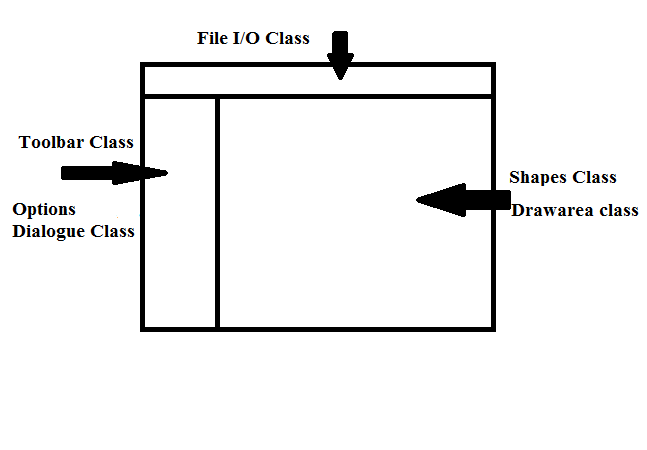
\includegraphics[scale=0.45]{architecture.png}
\end{figure}
\subsubsection{Developer{\textquoteright}s Architectural Rationale}
\subparagraph*{}{\selectlanguage{english}\color{black}
There are many reasons behind the selection of this structure. One is that 
it has been implemented in similar forms in other popular graphics tools. It is graphically 
similar to the layout of Paint, and other popular UML diagramming programs. It is also more modular to code, 
as different areas contain different responsibilities, and thus can be coded by individuals in their own time.}

\subsection[CONSISTENCY OF ARCHITECTURAL
VIEWS]{\selectlanguage{english}\bfseries\color{black} CONSISTENCY OF
ARCHITECTURAL VIEWS}
{\selectlanguage{english}\itshape\color{black}
For compliance with ISO/IEC 42010:2007 (�5.5) an Architectural
Description (AD) shall include a list of all known inconsistencies
between the architectural views and an analysis of consistency across
all the architectural views.}

\subsubsection{Detail of Inconsistencies between Architectural Views}
{\selectlanguage{english}\color{black}
There is consistency between the Architectural views, though the two focus on 
separate qualities. One inconsistency, however, is that the Developer's architecture
stresses the modularity of the code, without focusing much on the connections between the modules.
The user's code, however, focuses on how each section can be used in order to create a final product.}

\subsubsection{Consistency Analysis and Inconsistency Mitigations}
{\selectlanguage{english}\itshape\color{black}
A possible solution to the inconsistency listed above is to use group meetings to focus on creating a 
smooth connection between parts. If each member of the team works as efficiently as possible on their 
individual tasks, then the hours spent together can be to work out bugs between modules as they are linked
up to form the final program.}

\clearpage
\section{SOFTWARE DETAILED DESIGN}


\subsection[\ DEVELOPER{\textquoteright}S VIEWPOINT DETAILED SOFTWARE
DESIGN]{\foreignlanguage{english}{\ }\foreignlanguage{english}{DEVELOPER{\textquoteright}S
VIEWPOINT DETAILED SOFTWARE DESIGN}}

{\selectlanguage{english}\color{black}

A modular approach was preferred, separating the application into different distinct components that could operate independently. This allowed different developers to work on their own aspects of the program independently, with an emphasis on the Drawing Area, Toolbar/Options, and the Main Window, allowing the team to maximize work versus time.}
\begin{figure}[h!]
\caption{Topmost Class Diagram}
\centering
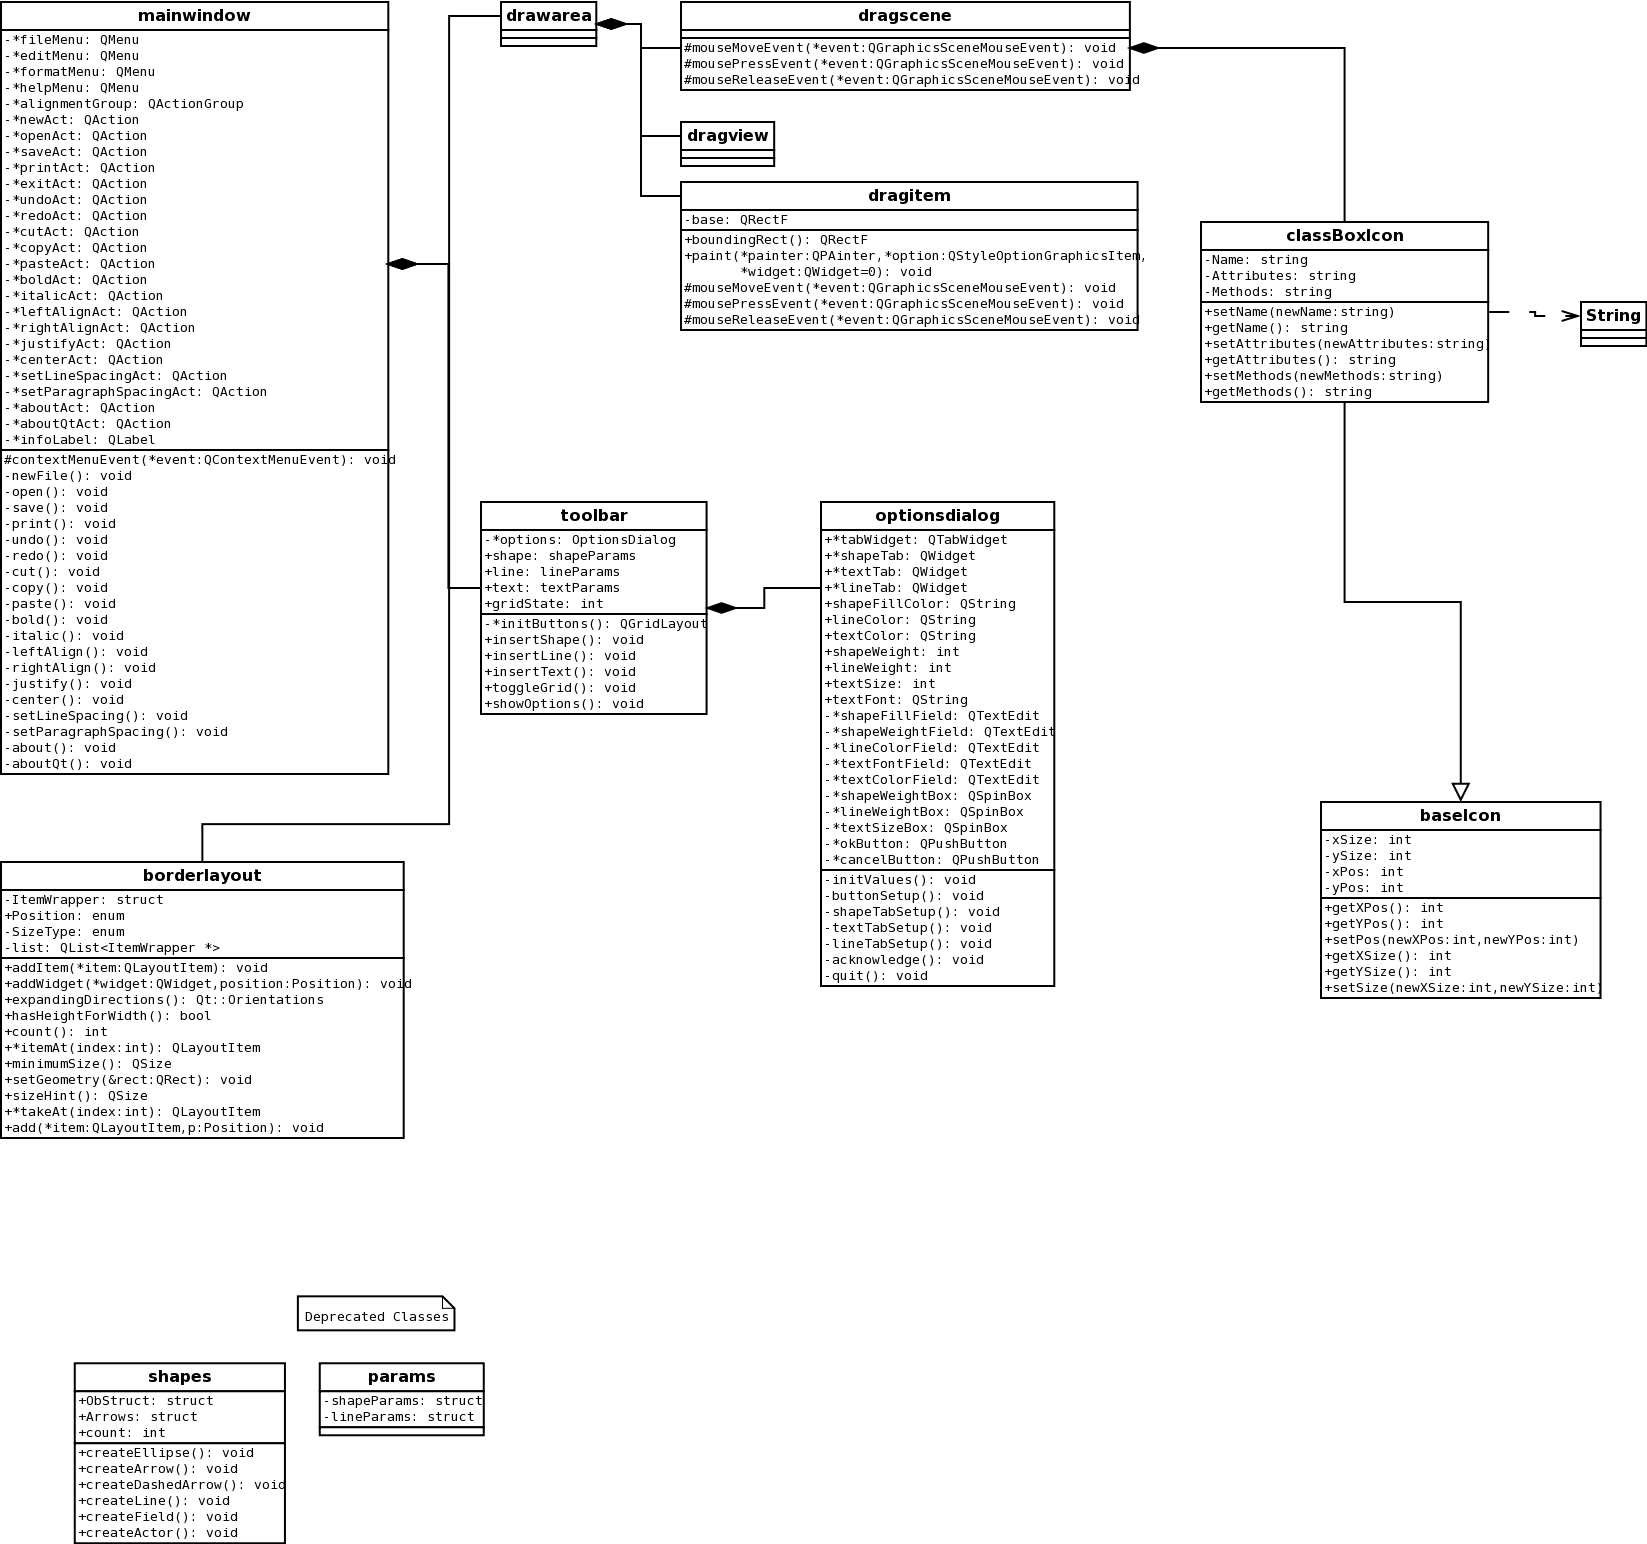
\includegraphics[width=\textwidth]{../UMLdiagrams/MasterClassDiagram.png}
\end{figure}
\subsection[COMPONENT/ENTITY
DICTIONARY]{\selectlanguage{english}\bfseries\color{black}
COMPONENT/ENTITY DICTIONARY}


{\selectlanguage{english}\itshape\color{black}
.
\begin{flushleft}
\tablehead{}
\begin{supertabular}{|m{1.0462599in}|m{0.9837598in}|m{1.6712599in}|m{1.2962599in}|m{1.2580599in}|}
\hline
\multicolumn{5}{|m{6.57056in}|}{\centering
\selectlanguage{english}\bfseries\color{black} Component/Entity
Dictionary}\\\hline
\centering \selectlanguage{english}\bfseries\color{black} Name &
\centering \selectlanguage{english}\bfseries\color{black} Type/Range &
\centering \selectlanguage{english}\bfseries\color{black}
Purpose/Function &
\centering \selectlanguage{english}\bfseries\color{black} Dependencies &
\centering\arraybslash \selectlanguage{english}\bfseries\color{black}
Subordinates\\\hline
~
MainWindow&
~
widget&
~
Manage overall layout&
~
none&
~
none
\\\hline
~
Drawing Area&
~
widget&
~
Create graphical view&
~
none&
~
none

\\\hline
~
Toolbar&
~
widget&
~
Manage buttons and change options&
~
Options Dialog&
~
none

\\\hline
\end{supertabular}
\end{flushleft}

\subsection[COMPONENT/ENTITY DETAILED
DESIGN]{\selectlanguage{english}\bfseries\color{black} COMPONENT/ENTITY
DETAILED DESIGN}
\subsubsection{Detailed Design for Component/Entity: MainWindow}
\paragraph[\ Introduction/Purpose of this
Component/Entity]{\ Introduction/Purpose of this Component/Entity}
{\selectlanguage{english}\color{black}
Manage the other components' positions and sizes in relation to each other. Will also terminate the other components when closed.}

\paragraph[Input for this Component/Entity]{Input for this
Component/Entity}
{\selectlanguage{english}\color{black}
User-generated resize/move/exit requests.}

\paragraph{Output for this Component/Entity}
{\selectlanguage{english}\color{black}
Positions and sizes for the other components.}

\paragraph{Component/Entity Process to Convert Input to Output}
{\selectlanguage{english}\color{black}
Calculate the appropriate sizes and positions based on a fixed ratio/layout.}

\paragraph{Design constraints and performance requirements of this
Component/Entity}
{\selectlanguage{english}\color{black}
None.}

\subsubsection{Detailed Design for Component/Entity: Drawing Area}
\paragraph[\ Introduction/Purpose of this
Component/Entity]{\ Introduction/Purpose of this Component/Entity}
{\selectlanguage{english}\color{black}
Create and show the appropriate representation of all the objects for the current file in a graphical view.}

\paragraph{Input for this Component/Entity}
{\selectlanguage{english}\color{black}
Position and size of new objects from the user, various aesthetic features, such as font and color, from the toolbar options.}

\paragraph{Output for this Component/Entity}
{\selectlanguage{english}\color{black}
Graphical representation of all currently existing shapes.}

\paragraph{Component/Entity Process to Convert Input to Output}
{\selectlanguage{english}\color{black}
Call object creation functions from shapes with the appropriate parameters, which will then handle object creation and return an appropriate reference, to be used in drawing the object.}

\paragraph{Design constraints and performance requirements of this
Component/Entity}
{\selectlanguage{english}\color{black}
None.}

\subsubsection{Detailed Design for Component/Entity: Toolbar}
\paragraph[\ Introduction/Purpose of this
Component/Entity]{\ Introduction/Purpose of this Component/Entity}
{\selectlanguage{english}\color{black}
Manage buttons for creating the various shapes, making sure that the specified shape is appropriate for the current diagram type. It will also manage the grid state, as well as default options, such as font, weight, or color.}

\paragraph{Input for this Component/Entity}
{\selectlanguage{english}\color{black}
User pushing a specific button, selecting new option values, or toggling the grid.}

\paragraph{Output for this Component/Entity}
{\selectlanguage{english}\color{black}
Button presses will signal the appropriate function, such as create new shape, save, or load. Changing the default options will result in all new shapes being created with those parameters. Toggling the grid will result in the grid becoming visible or invisible.}

\paragraph{Component/Entity Process to Convert Input to Output}
{\selectlanguage{english}\color{black}
For creating new shapes, the Toolbar will send a request to make a new object of the specified type. For options, the Toolbar will open an Option Dialog and allow the user to specify new changes, saving those changes when confirmation is received. For other buttons, appropriate functions will be called, signalling MainWindow or DrawArea if needed.}

\paragraph{Design constraints and performance requirements of this
Component/Entity}
{\selectlanguage{english}\color{black}
None.}


\subsection{DATA DICTIONARY}


\begin{flushleft}
\tablehead{}
\begin{supertabular}{|m{0.9837598in}|m{0.9212598in}|m{1.8587599in}|m{1.2962599in}|m{1.1330599in}|}
\hline
\multicolumn{5}{|m{6.50806in}|}{\centering
\selectlanguage{english}\bfseries\color{black} Data Dictionary}\\\hline
\centering \selectlanguage{english}\bfseries\color{black} Name &
\centering \selectlanguage{english}\bfseries\color{black} Type/Range &
\centering \selectlanguage{english}\bfseries\color{black} Defined
by{\dots} &
\centering \selectlanguage{english}\bfseries\color{black} Referenced
by{\dots} &
\centering\arraybslash \selectlanguage{english}\bfseries\color{black}
Modified by{\dots}\\\hline
~
ObStruct&
~
Data Structure&
~
shapes.h&
~
drawArea.cpp&
~
none
\\\hline
~
Arrows&
~
Data Structure&
~
shapes.h&
~
drawArea.cpp&
~
none
\\\hline
~
OptionsDialog&
~
QDialog&
~
optionsDialog.h&
~
toolbar.cpp&
~
Toolbar
\\\hline
\end{supertabular}
\end{flushleft}
%\clearpage\setcounter{page}{1}\pagestyle{Convertvii}
\section[REQUIREMENTS
TRACEABILITY]{\selectlanguage{english}\bfseries\color{black}
REQUIREMENTS TRACEABILITY}
{\selectlanguage{english}\color{black}
\foreignlanguage{english}{\textit{This section shall contain
traceability information from each system requirement in this
specification to the system (or subsystem, if applicable) requirements
it addresses. \ A tabular form is preferred, but not mandatory.
}}\foreignlanguage{english}{\textit{A detailed mapping between
requirements and constraints in the SSRS and architectural components
and detailed entities in this SSDD is required. For compliance with
ISO/IEC 15288:2008
}}\foreignlanguage{english}{\textit{(�6.4.3.3.c)}}\foreignlanguage{english}{\textit{
an Architectural Description (AD) shall provide roundtrip traceability
between the system and software requirements and the architectural
design entities. All requirements and constraints within the SSRS shall
map to a set of architectural entities. All entities in all the
architectural views shall be associated with either a requirement or
constraint in the SSRS or an architectural constraint within this
SSDD.}}}

\bigskip
\begin{flushleft}
\tablehead{%
\hline
Req No. & SDD & Alpha Test Results \\\hline}
\begin{supertabular}{|m{1.5in}|m{0.6in}|m{4.0in}|}
UC1 &  & F \\\hline
UC2 & & F \\\hline
UC3 & & F \\\hline
UC4 & & F \\\hline
UC5 & & F \\\hline
UC6 & & 50\% - grid displays, but button does not toggle \\\hline
UC7 & & 30\% - several shapes can be placed \\\hline
UC8 & & F \\\hline
UC9 & & F \\\hline
UC10 & & F \\\hline


Select shapes & UC11 & The user selects the shapes for further commands.
\\\hline
Move shapes & UC12 & The user moves the shapes to a different location on the drawing area. 
\\\hline
Copy shapes & UC13 & The user copies the selected shapes to the clipboard.
\\\hline
Cut shapes & UC14 & The user cuts the selected shapes to the clipboard. The shapes are removed from the drawing area.
\\\hline
Paste shapes & UC15 & The user pastes the shapes from the clipboard into the drawing area.
\\\hline
Edit shape properties & UC16 & The user edits a shape on the drawing area.
\\\hline
Edit default properties & UC17 & The user edits the default properties of the UML tool.
\\\hline
\end{supertabular}
\end{flushleft}

{\selectlanguage{english}\color{black}
Priorities are: \textbf{M}andatory, \textbf{L}ow, \textbf{H}igh}

{\selectlanguage{english}\color{black}
SDD link is version and page number or function name.}

{\selectlanguage{english}\color{black}
Test cases and results are file names and \textbf{P}ass/\textbf{F}ail or
\% passing.}

\end{document}
